\documentclass[11pt, oneside, dvipdfmx]{book}
\newcommand{\folder}{/usr/local/share/texmf}
%\newcommand{\folder}{/home/hanchenggao/Documents/texmf}
\input{\folder/hfiles/ebook}
%\usepackage[ruled,vlined]{algorithm2e}
\usepackage {graphicx}[dvips]
%\usepackage {graphics}
%\setCJKmainfont{SimSun}
\title{
Input-Structure Distance spectrum based on RTZ and Parity-check sequences of weight 2}
\author{Kwame Ackah Bohulu}
\date{\today}
\begin{document}

\maketitle

\newpage
\section{Input-Structure Distance spectrum based on RTZ and Parity-check sequences of weight 2}

\paragraph{5/7 RSC code, $f(x)=1+x^2,~g(x)=1+x+x^2$ \newline}
$f(x)$ is Case3 whiles $g(x)$ is Case1
if $a(x)=\frac{h(x)}{f(x)},~a(x)=\sum_{i=1}^{I}x^{a-2i}$

if $a(x)=\frac{b(x)}{g(x)},~a(x)=\sum_{i=1}^{I}x^{b-3i+1}+x^{b-3i}$
 \begin{table*}[h!]
 \caption{$a(x),~b(x)$ for $h(x)=1+x^a$ generated via $f(x).~d_{\text{max}}=8$}
\centering
 \begin{tabular}{c c c} 
 \hline
 $a(x)$ & $b(x)$ & $h(x)$ \\ [0.5ex] 
 \hline\hline
$1$ & $1+x+x^{2}$ & $1+x^2$\\
\hline
$1+x^2$ & $1+x+x^3+x^4$ & $1+x^{4}$\\
\hline
$1+x^2+x^4$ & $1+x+x^3+x^5+x^6$ &  $1+x^{6}$\\
\hline
$1+x^2+x^4+x^6$ & $1+x+x^3+x^5+x^7+x^8$ &  $1+x^{8}$\\
 \end{tabular}
 \label{Tab1}
\end{table*}

 \begin{table*}[h!]
 \caption{$a(x),~h(x)$ for $b(x)=1+x^b$ generated via $g(x).~d_{\text{max}}=8$}
\centering
 \begin{tabular}{c c c} 
 \hline
 $a(x)$ & $b(x)$ & $h(x)$ \\ [0.5ex] 
 \hline\hline
$1+x$ & $1+x^{3}$ & $1+x+x^2+x^3$\\
\hline
$1+x+x^3+x^4$ & $1+x^6$ & $1+x+x^{2}+x^4+x^5+x^6$\\
 \end{tabular}
 \label{Tab2}
\end{table*}

\begin{figure}[h]
\centering
		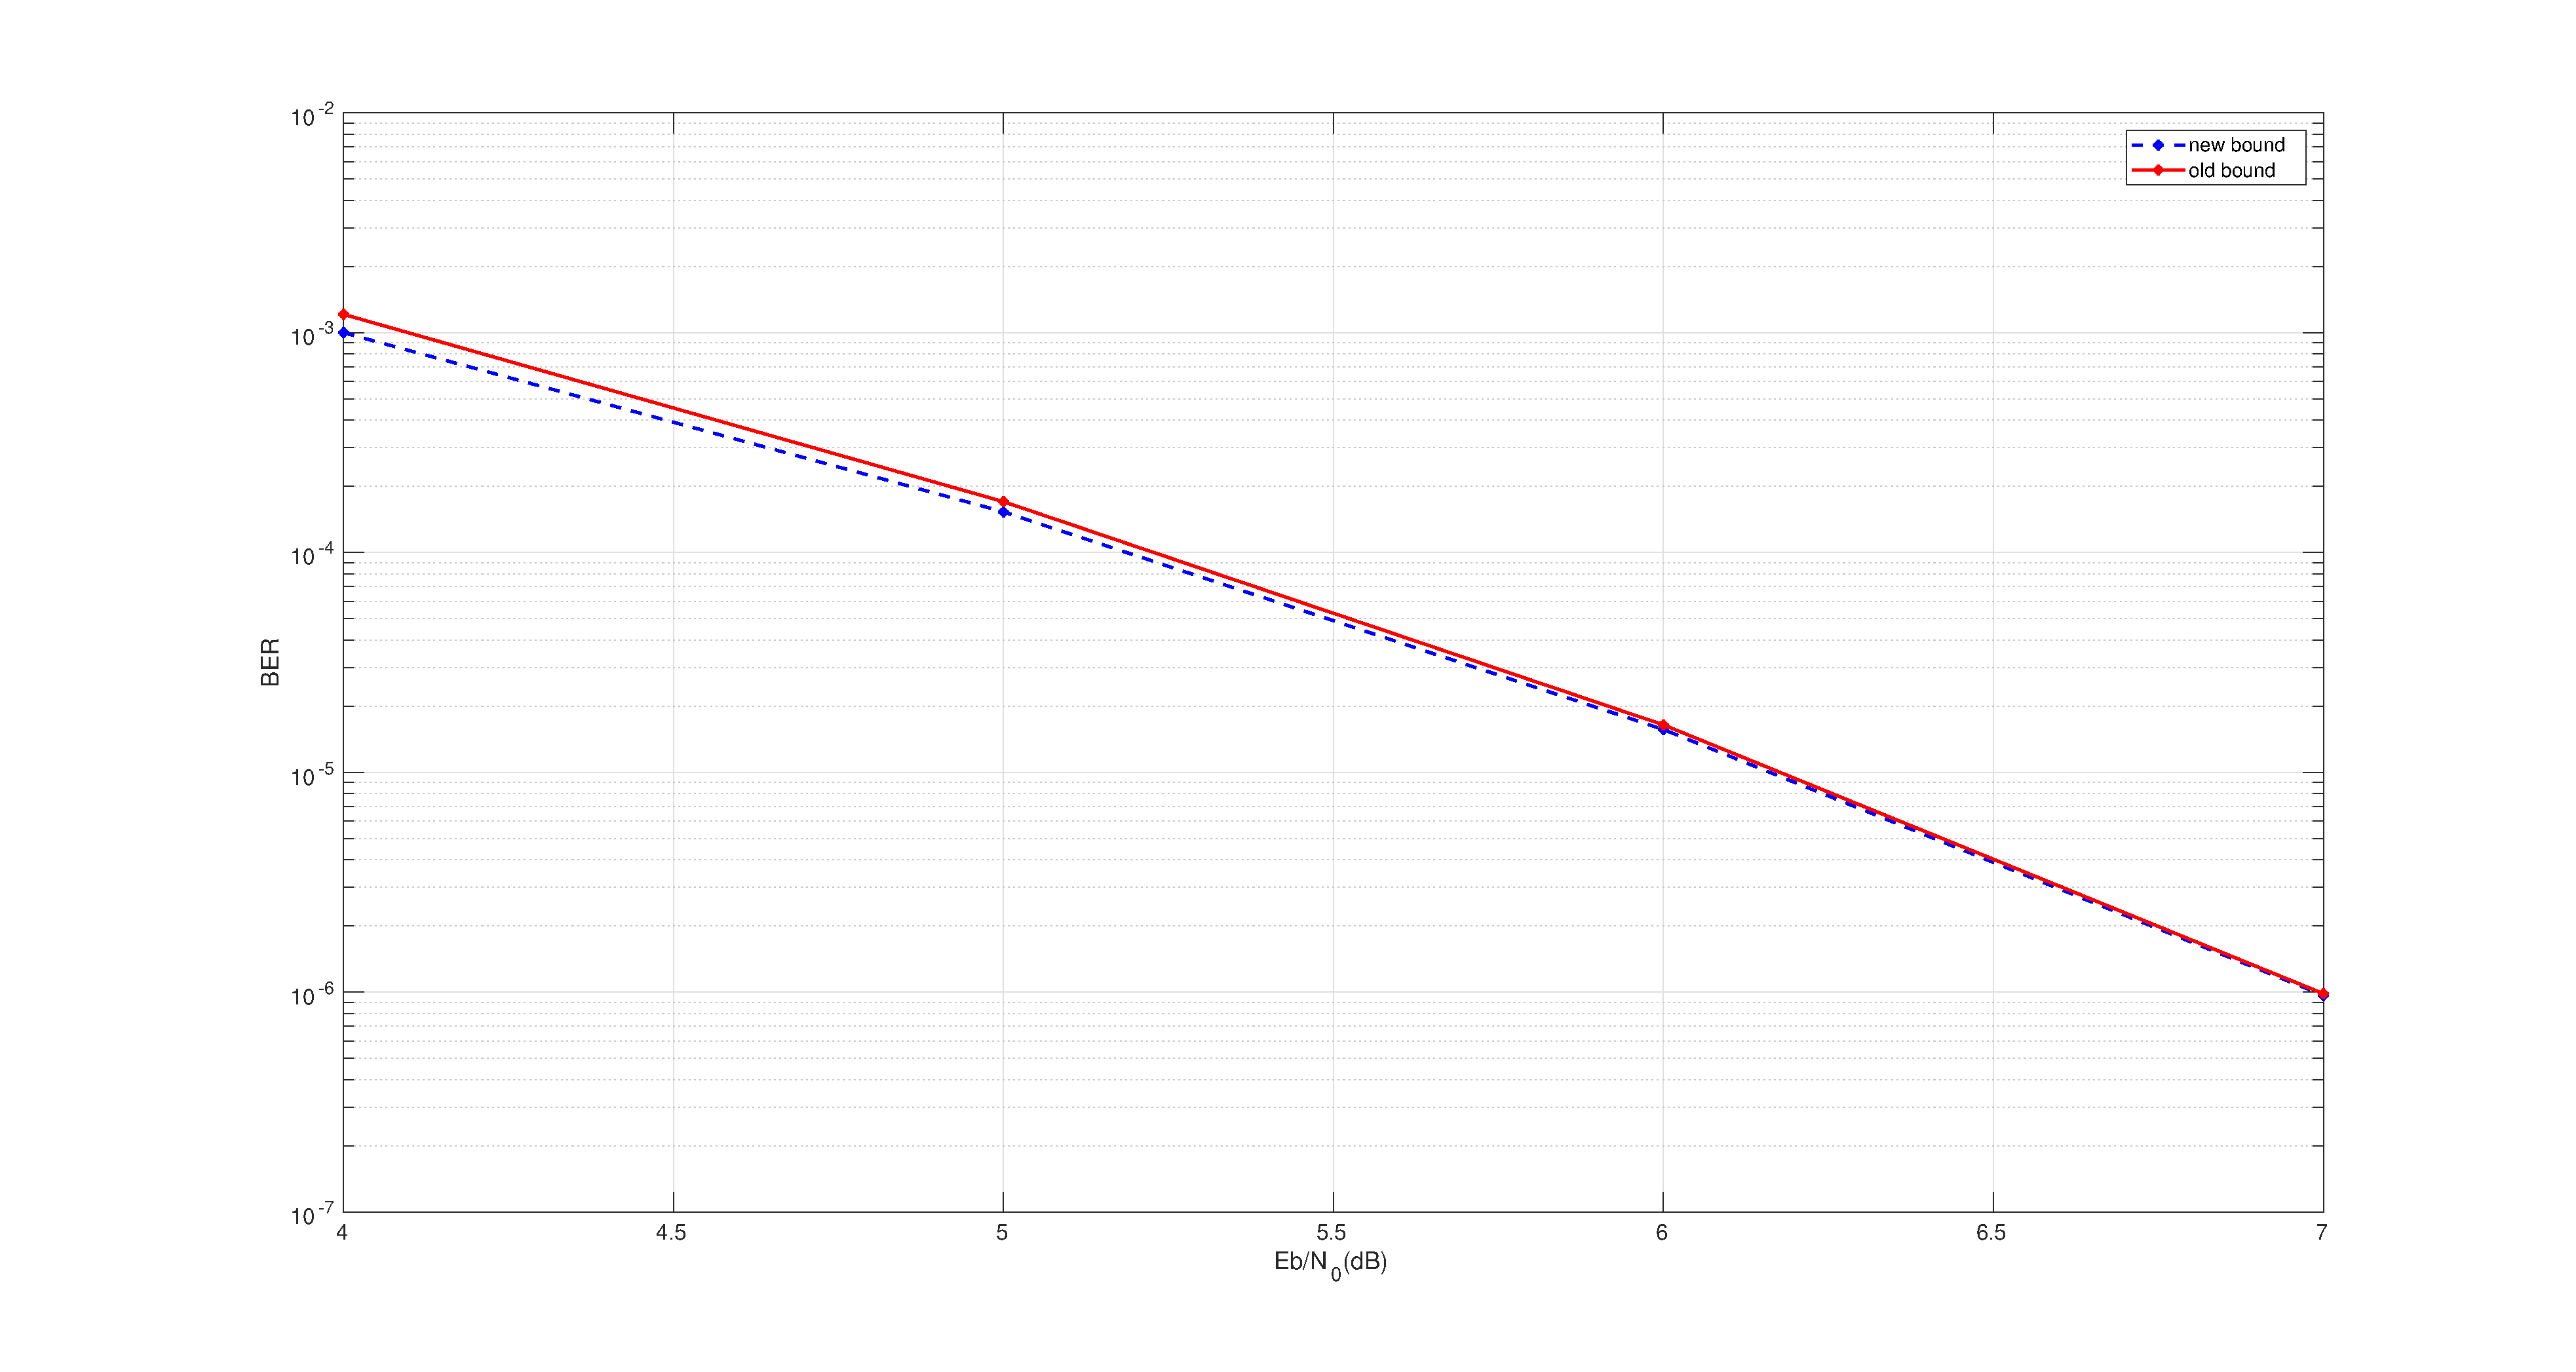
\includegraphics[width=\textwidth]{./Images/RSC_5_7.eps}
		\caption{Old Bound vs New Bound for 5/7 RSC Code}
		\label{fig1}
		\end{figure}


\newpage
%=============================
\paragraph{37/21 RSC code, $f(x)=1+x+x^2+x^3+x^4,~g(x)=1+x^4$ \newline}
$f(x)$ is Case2 whiles $g(x)$ is Case3

if $a(x)=\frac{h(x)}{f(x)},~a(x)=\sum_{i=1}^{I}x^{b-5i+1}+x^{b-5i}$

if $a(x)=\frac{b(x)}{g(x)},~a(x)=\sum_{i=1}^{I}x^{b-4i}
$

\begin{table*}[h!]
 \caption{$a(x),~b(x)$ for $h(x)=1+x^a$ generated via $f(x).~d_{\text{max}}=9$}
\centering
 \begin{tabular}{c c c} 
 \hline
 $a(x)$ & $b(x)$ & $h(x)$ \\ [0.5ex] 
 \hline\hline
$1+x$ & $1+x+x^{4}+x^5$ & $1+x^5$\\
\hline
$1+x+x^5+x^6$ & $1+x+x^4+x^6+x^{9}+x^{10}$ & $1+x^{10}$\\
%\hline
%$1+x+x^5+x^6+x^{10}+x^{11}$ & $1+x+x^4+x^6+x^{9}+x^{11}+x^{14}+x^{15}$ & $1+x^{15}$\\
 \end{tabular}
 \label{Tab3}
\end{table*}

 \begin{table*}[h!]
 \caption{$a(x),~h(x)$ for $b(x)=1+x^b$ generated via $g(x).~d_{\text{max}}=9$}
\centering
 \begin{tabular}{c c c} 
 \hline
 $a(x)$ & $b(x)$ & $h(x)$ \\ [0.5ex] 
 \hline\hline
$1$ & $1+x^{4}$ & $1+x+x^2+x^3+x^4$\\
 \end{tabular}
 \label{Tab4}
\end{table*}

\begin{figure}[h]
\centering
		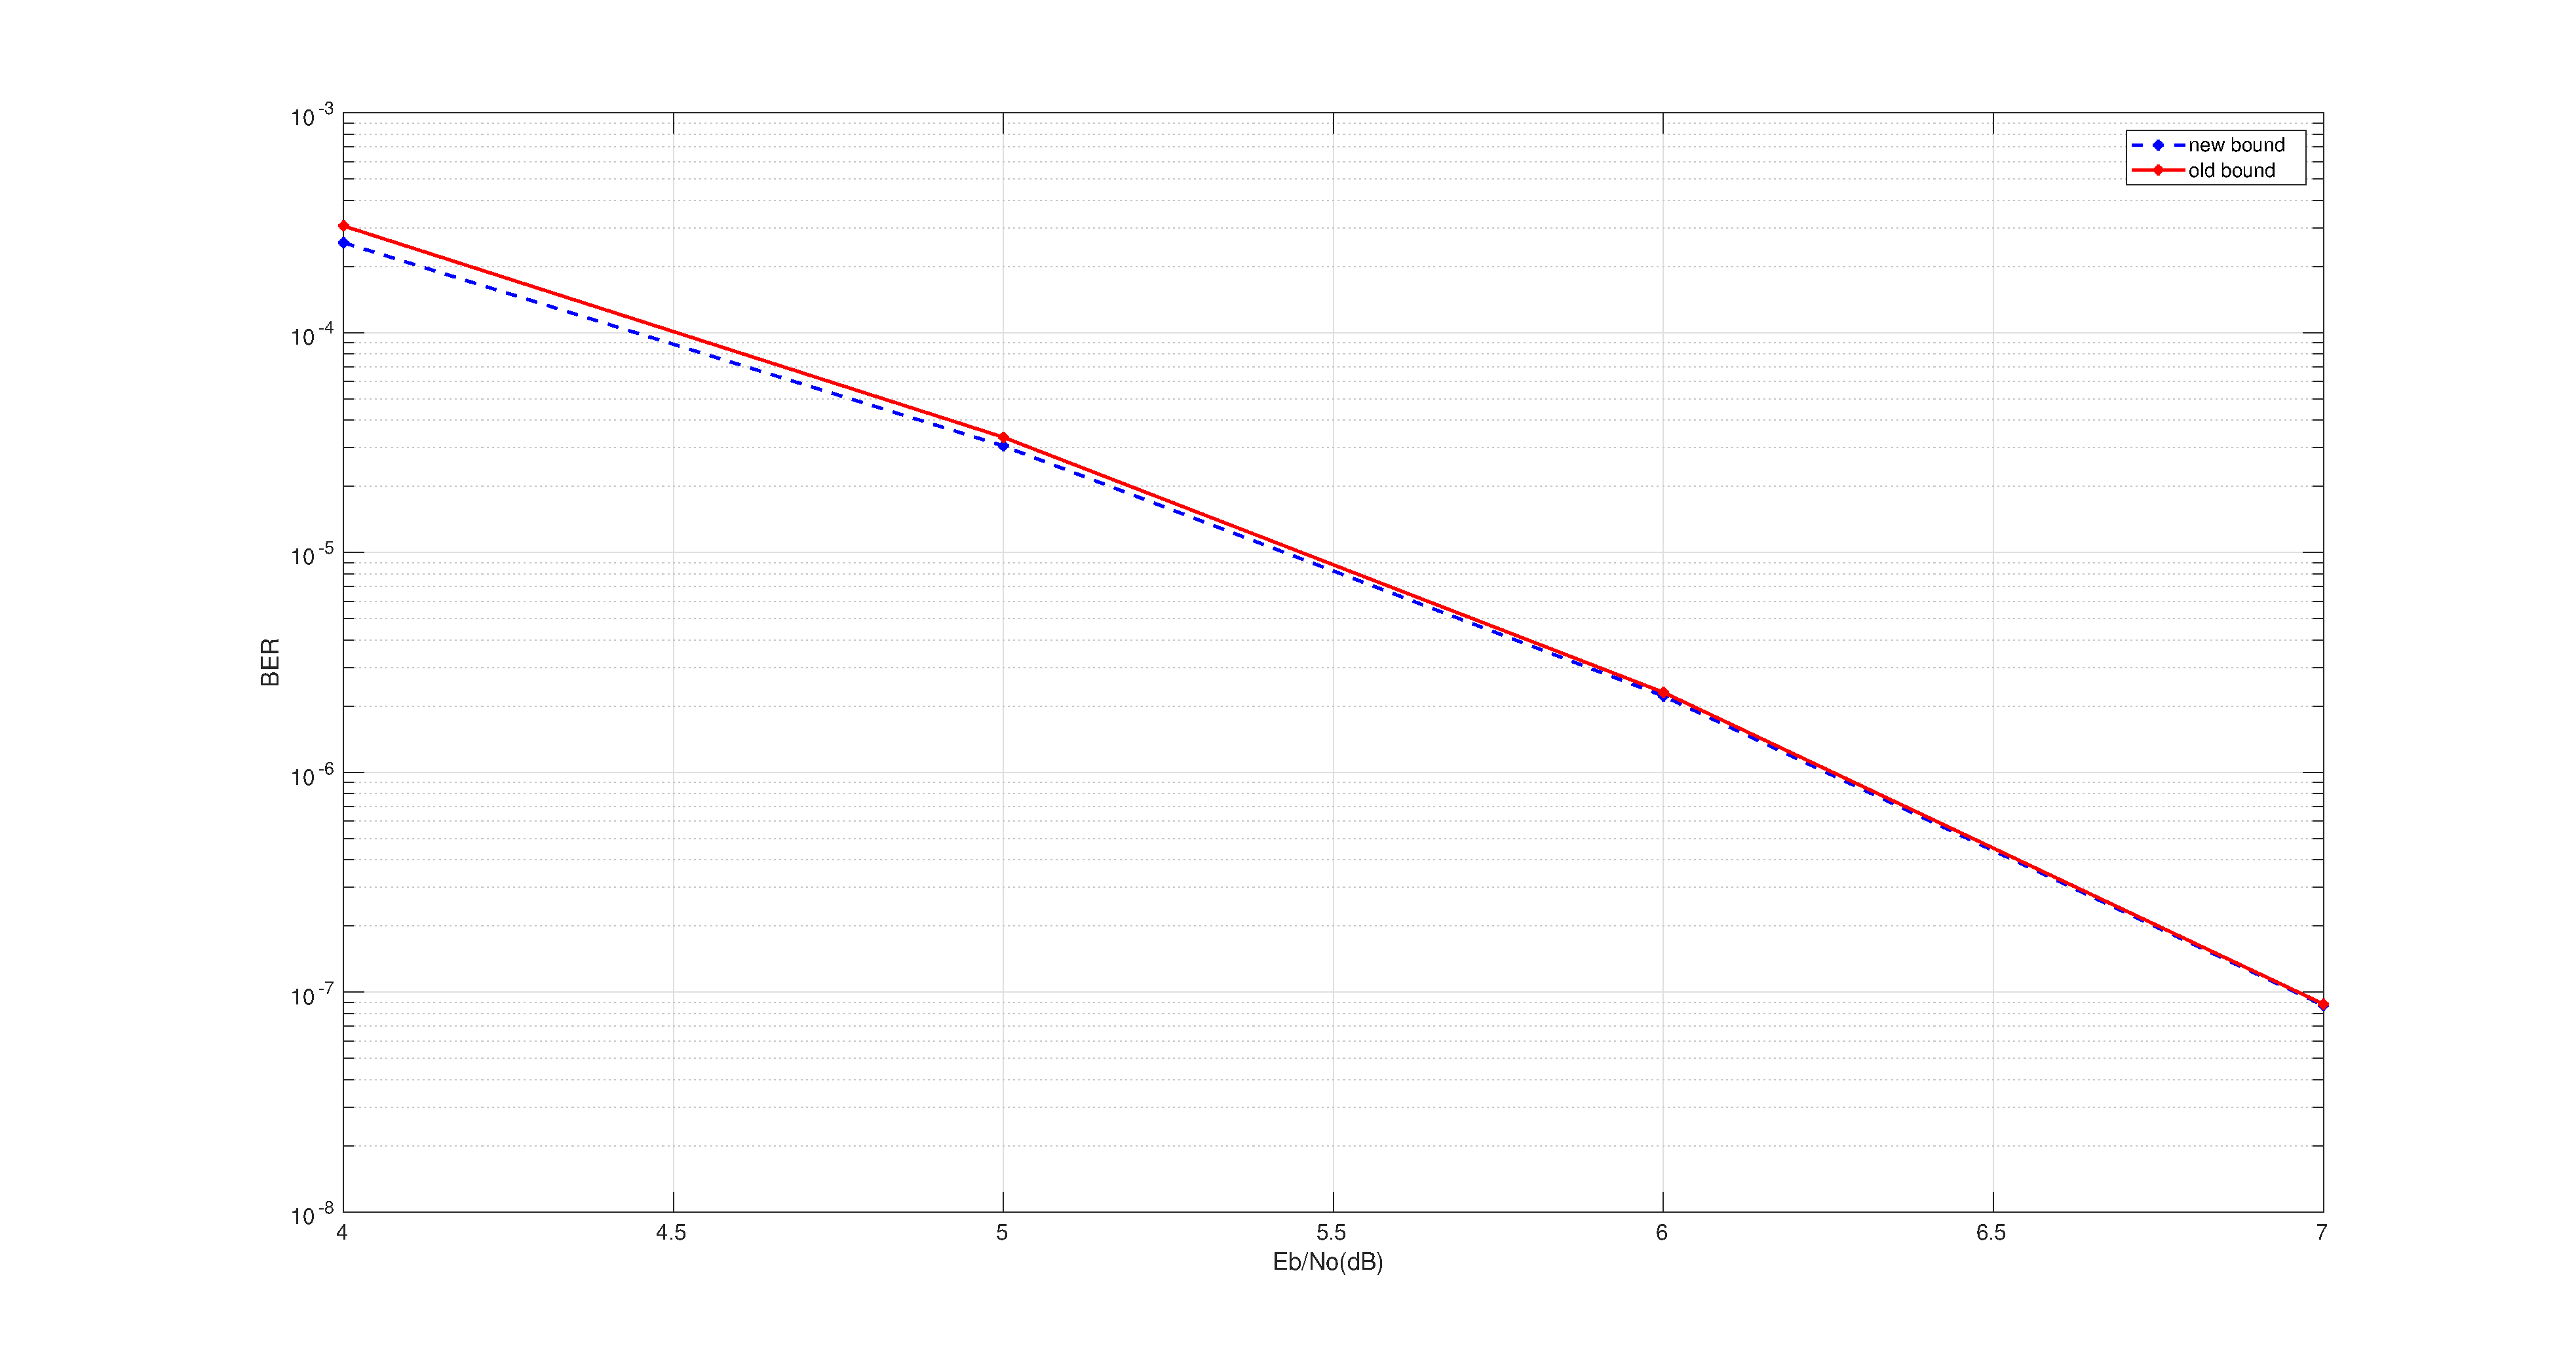
\includegraphics[width=\textwidth]{./Images/RSC_37_21.eps}
		\caption{Old Bound vs New Bound for 37/21 RSC Code}
		\label{fig2}
		\end{figure}
%================================
\newpage
\paragraph{23/35 RSC code, $f(x)=1+x+x^4,~g(x)=1+x^2+x^3+x^4$ \newline}
$f(x)$ is Case1 whiles $g(x)$ is Case4

if $a(x)=\frac{b(x)}{g(x)},~a(x)=\sum_{i=1}^{I}x^{b-7i+3}+x^{b-7i+2}+x^{b-7i}$

\begin{table*}[h!]
 \caption{$a(x),~b(x)$ for $h(x)=1+x^a$ generated via $f(x).~d_{\text{max}}=10$}
\centering
 \begin{tabular}{c c c} 
 \hline
 $a(x)$ & $b(x)$ & $h(x)$ \\ [0.5ex] 
 \hline\hline
$~-~$ & $~-~$ & $~-~$\\

 \end{tabular}
 \label{Tab5}
\end{table*}

 \begin{table*}[h!]
 \caption{$a(x),~h(x)$ for $b(x)=1+x^b$ generated via $g(x).~d_{\text{max}}=10$}
\centering
 \begin{tabular}{c c c} 
 \hline
 $a(x)$ & $b(x)$ & $h(x)$ \\ [0.5ex] 
 \hline\hline
$1+x^2+x^3$ & $1+x^{7}$ & $1+x+x^2+x^6+x^7$\\
\hline
$1+x^2+x^3+x^7+x^9+x^{10}$ & $1+x^{14}$ & $1+x+x^2+x^6+x^8+x^9+x^{13}+x^{14}$\\
 \end{tabular}
 \label{Tab6}
\end{table*}

\begin{figure}[h]
\centering
		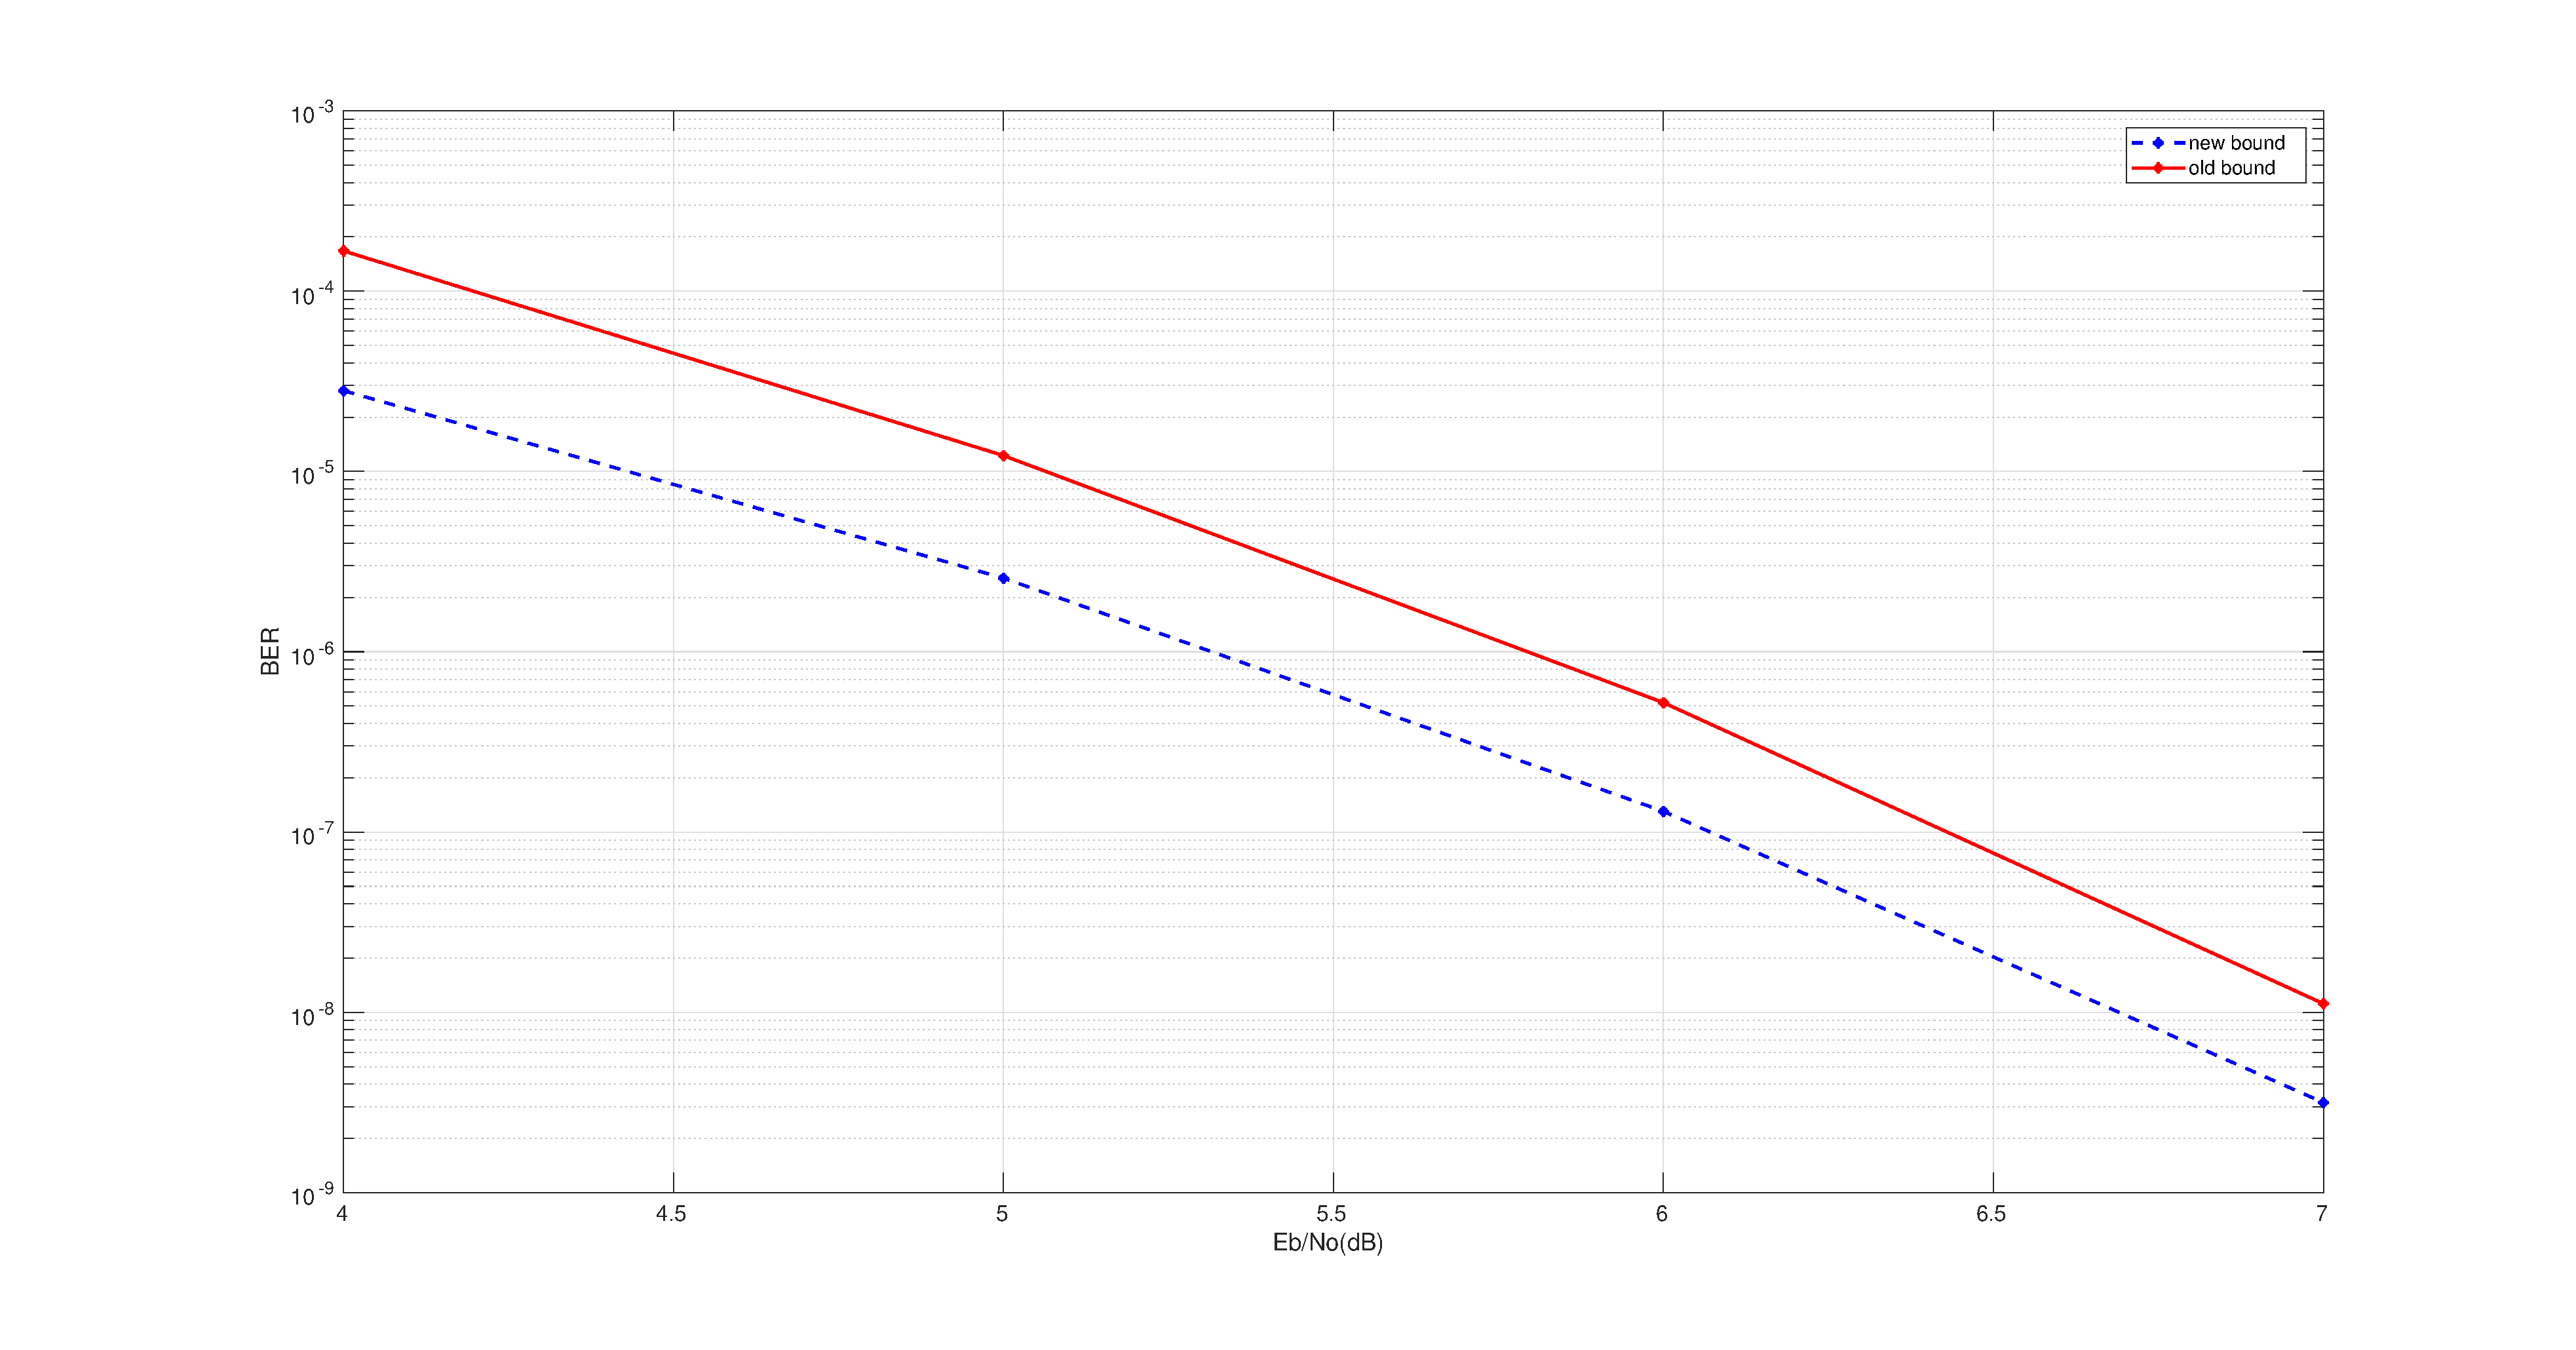
\includegraphics[width=\textwidth]{./Images/RSC_23_35.eps}
		\caption{Old Bound vs New Bound for 23/35 RSC Code}
		\label{fig3}
		\end{figure}
	
	\newpage	
\section{List of Weight3 Parity-Check Sequences}	
It looks like $h(x)$ has a weight 3 Structure of the form $1+x^a+x^b$ iff $f(x)$ has an odd number of terms $\geq 3$.

\begin{enumerate}
\item $f(x)$ is a single primitive polynomial, eg $f(x)=1+x+x^2$.
\begin{table*}[h!]
 \caption{$f(x)=1+x+x^2$}
\centering
 \begin{tabular}{c c} 
 \hline
 $a(x)$ & $h(x)$ \\ [0.5ex] 
 \hline\hline
$1$ & $1+x+x^2$\\
\hline
$1+x+x^2$  & $1+x^2+x^4$\\
\hline
$1+x+x^3$  & $1+x^4+x^5$\\
\hline
$1+x^2+x^3$  & $1+x+x^5$\\
\hline
$1+x+x^2+x^4+x^5$  & $1+x^2+x^7$\\
\hline
$1+x+x^3+x^4+x^5$  & $1+x^5+x^7$\\
\hline
$1+x+x^3+x^4+x^6$  & $1+x^7+x^8$\\
 \end{tabular}
 \label{Tab7a}
\end{table*}

\begin{table*}[h!]
 \caption{$f(x)=1+x+x^4$}
\centering
 \begin{tabular}{c c} 
 \hline
 $a(x)$ & $h(x)$ \\ [0.5ex] 
 \hline\hline
$1$ & $1+x+x^4$\\
\hline
$1+x+x^2+x^3+x^5$  & $1+x^7+x^9$\\
\hline
$1+x+x^2+x^3+x^5+x^7+x^8$  & $1+x^{11}+x^{12}$\\
\hline
$1+x+x^4$  & $1+x^{2}+x^{8}$\\
\hline
$1+x+x^2+x^4+x^6+x^7+x^{10}$  & $1+x^3+x^{14}$\\
\hline
$1+x+x^2+x^3+x^6$  & $1+x^5+x^{10}$\\
\hline
$1+x+x^2+x^3+x^5+x^6+x^9$  & $1+x^{6}+x^{13}$\\
\hline
$1+x+x^2+x^3+x^4+x^6+x^8+x^9+x^{12}$  & $1+x^4+x^{16}$\\
\hline
$1+x+x^2+x^3+x^5+x^7+x^9+x^{10}+x^{13}$  & $1+x^8+x^{17}$\\
\hline
$1+x+x^2+x^3+x^5+x^7+x^8+x^{11}+x^{14}$  & $1+x^{14}+x^{18}$\\
 \end{tabular}
 \label{Tab7b}
\end{table*}


\item $f(x)$ is prime but not a primitive polynomial, eg $f(x)=1+x+x^2+x^3+x^4$
Could not find any parity-check bits with weight 3

\item $f(x)$ is made up of equal repeated polynomial roots, eg $f(x)=1+x^2+x^4=(1+x+x^2)^2$.

\begin{table*}[h!]
 \caption{$f(x)=1+x^2+x^4$}
\centering
 \begin{tabular}{c c} 
 \hline
 $a(x)$ & $h(x)$ \\ [0.5ex] 
 \hline\hline
$1$ & $1+x^2+x^4$\\
\hline
$1+x^2+x^4$  & $1+x^2+x^4$\\
\hline
$1+x^2+x^6$  & $1+x^8+x^{10}$\\
\hline
$1+x^4+x^6$  & $1+x^2+x^{10}$\\
\hline
$1+x^2+x^4+x^8+x^{10}$  & $1+x^4+x^{14}$\\
\hline
$1+x^2+x^{6}+x^{8}+x^{10}$  & $1+x^{10}+x^{14}$\\
 \end{tabular}
 \label{Tab8}
\end{table*}

\item  $f(x)$ is made up of unique repeated polynomial roots.
\end{enumerate}	
		
\end{document}